\documentclass[a4paper, 10pt, dvipdfmx]{jlreq}

\usepackage{amsmath,amsfonts,amssymb}
\usepackage{bm}
\usepackage{mathtools}
\usepackage{siunitx}
\usepackage[dvipdfmx]{graphicx}
\usepackage[dvipdfmx]{color}
\usepackage[dvipdfmx, colorlinks=true, allcolors=blue]{hyperref}
\usepackage{listings, jlisting}
\usepackage{tikz}
\usepackage{physics}
\usepackage{url}

\Urlmuskip=0mu plus 10mu
\allowdisplaybreaks[4]
\frenchspacing
\definecolor{OliveGreen}{rgb}{0.0,0.6,0.0}
\definecolor{Orenge}{rgb}{0.89,0.55,0}
\definecolor{SkyBlue}{rgb}{0.28, 0.28, 0.95}
\lstset{
  language={c++},
  basicstyle={\ttfamily},
  identifierstyle={\small},
  ndkeywordstyle={\small},
  frame=single,
  breaklines=true,
  numbers=left,
  xrightmargin=0zw,
  xleftmargin=3zw,
  numberstyle={\scriptsize},
  lineskip=-0.9ex,
  keywordstyle={\small\bfseries\color{SkyBlue}},
  commentstyle={\color{OliveGreen}},
  stringstyle={\small\ttfamily\color{Orenge}}
}

\begin{document}

\title{k-RDMの高速化手法について}
\author{計数工学科 3 年 03-220602 浜口広樹}
\date{\today}
\maketitle

\section*{fda}

実は、上記のことを考えずとも、今回の$C_i$に対しては、任意個の重複がない行列積が直接求まります。

まず、行列$C_i$の定義を述べます。以下、$\mathbb{N}$は$0$を含むものとします。

関数$f(i,ps) : \mathbb{N} \times \mathbb{N}^\mathbb{N} \to \pm 1$を以下の様に定義します。

$$
    f(i,ps)=\sum_{p \in ps}{popcount\left(i>>p\right)}
$$

ただし、関数$popcount(i): \mathbb{N} \to \mathbb{N}$は、$i$を二進数表記した際の1の個数(立っているビット数)とし、
$i>>p$で$i$を$p$桁右シフトした値($\left\lfloor\frac{i}{2^p}\right\rfloor$)を表すものとします。

\begin{figure}[htbp]
    \begin{minipage}{0.45\hsize}
        \begin{center}
            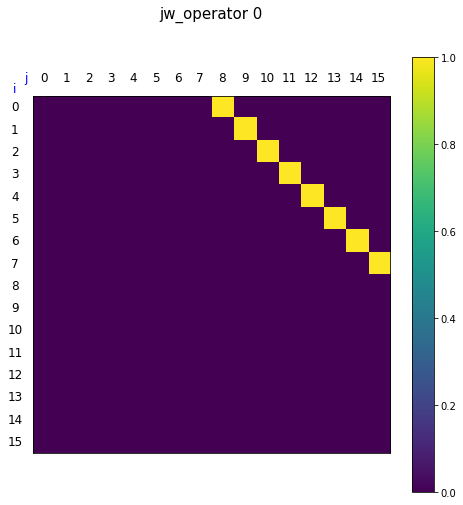
\includegraphics[width=70mm]{jw_operators/0.png}
        \end{center}
        \caption{0番目}
    \end{minipage}
    \begin{minipage}{0.45\hsize}
        \begin{center}
            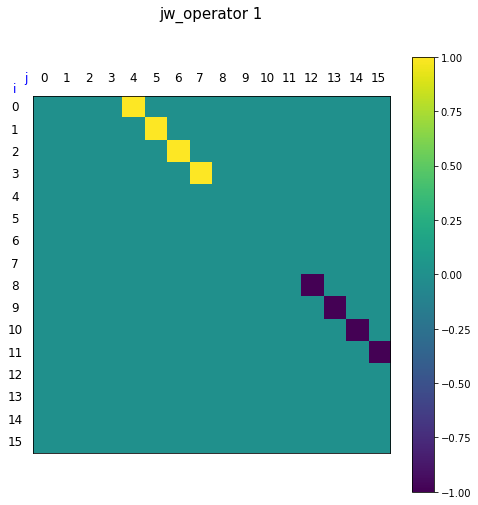
\includegraphics[width=70mm]{jw_operators/1.png}
        \end{center}
        \caption{1番目}
    \end{minipage}
\end{figure}
\begin{figure}[htbp]
    \begin{minipage}{0.45\hsize}
        \begin{center}
            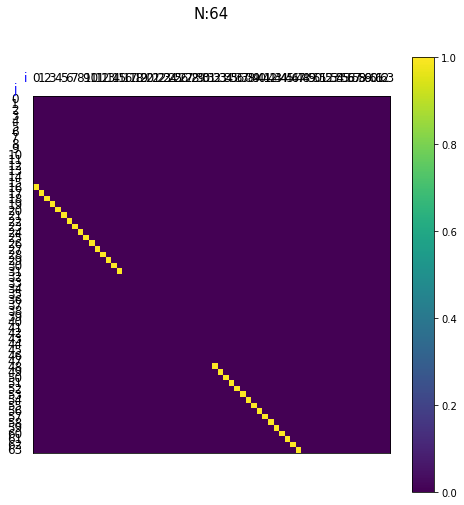
\includegraphics[width=70mm]{jw_operators/2.png}
        \end{center}
        \caption{2番目}
    \end{minipage}
    \begin{minipage}{0.45\hsize}
        \begin{center}
            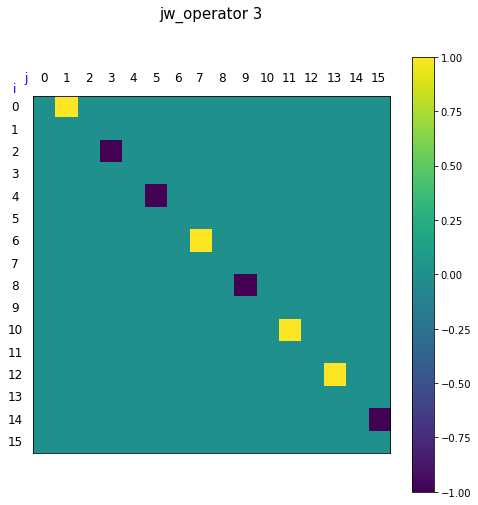
\includegraphics[width=70mm]{jw_operators/3.png}
        \end{center}
        \caption{3番目}
    \end{minipage}
\end{figure}

\end{document}

